\chapter{Síntese total: estratégia e rotas clássicas}\label{ch:b3:total-synthesis}

O fármaco anticâncer paclitaxel foi isolado pela primeira vez da casca do teixo do
Pacífico, uma árvore de crescimento lento; retirar a casca matava a árvore, e o suprimento
ficava muito aquém do que os pacientes precisavam. Os químicos responderam de duas maneiras: sínteses
totais, que mostraram que a molécula podia ser construída a partir de materiais de partida
simples, mas eram longas demais para a produção, e uma \omterm{def:b3:total-synthesis:total}{semissíntese} a partir de um
composto aparentado extraído das folhas de um teixo comum, que é renovável.
Este capítulo trata de como essas rotas são avaliadas e planejadas: como os rendimentos
se multiplicam, por que a convergência compensa, quanto custam os grupos protetores, que ligações
formar primeiro, e três sínteses marcantes lidas com essas ferramentas.

\begin{recall}
O volume do 2.º ano tratou da análise retrossintética (molécula-alvo,
desconexão, síntons, equivalente sintético, interconversão de grupos
funcionais), dos grupos protetores ortogonais, da reação aldólica, da
anelação de Robinson, da reação de Wittig e da química dos íons imínio; o volume do 1.º
ano, dos grupos protetores e dos rendimentos. O \cref{ch:b3:asymmetric-synthesis},
o \cref{ch:b3:pericyclic} e o \cref{ch:b3:homogeneous-catalysis} forneceram as
etapas-chave modernas.
\end{recall}

\begin{omfigure}
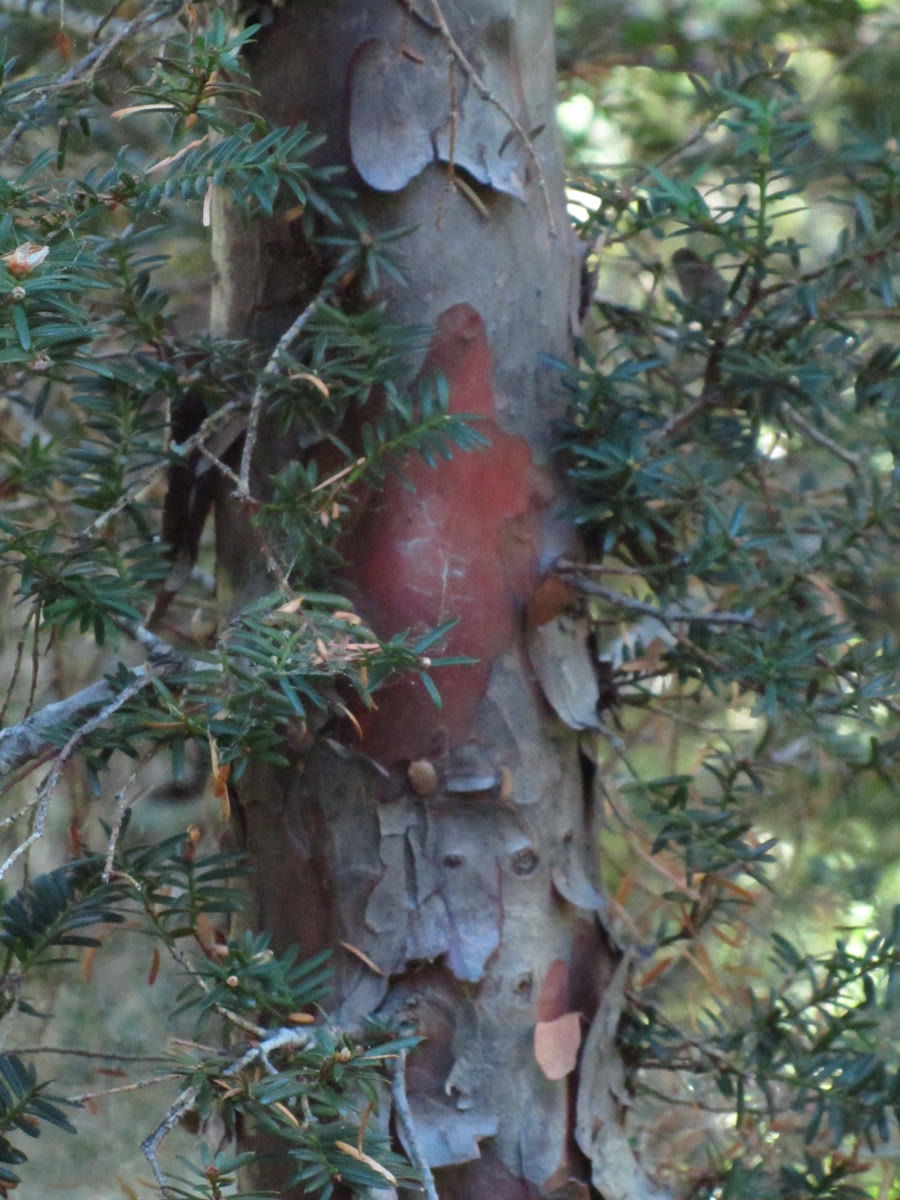
\includegraphics[width=0.32\linewidth]{images/book4/pacific-yew.jpg}

{\small Casca e folhas de um teixo do Pacífico, a primeira fonte de paclitaxel.
Fotografia: JOE BLOWE, CC BY-SA 2.0.}
\end{omfigure}

\section{Medir uma síntese}

\begin{definition}[Síntese total]\label{def:b3:total-synthesis:total}
Uma \emph{síntese total}\index{sintese total@síntese total} produz uma molécula complexa, muitas vezes
um produto natural, a partir de compostos comerciais simples. Uma \emph{síntese
formal}\index{sintese formal@síntese formal} produz um intermediário de uma síntese total
anterior, completando a rota no papel. Uma \emph{semissíntese}\index{semissintese@semissíntese}
parte de um composto natural já próximo do alvo.
\end{definition}

\begin{definition}[Arquitetura de uma rota]\label{def:b3:total-synthesis:architecture}
Em uma \emph{síntese linear}\index{sintese linear@síntese linear}, cada etapa age sobre o
produto da anterior; em uma \emph{síntese convergente}\index{sintese convergente@síntese convergente},
fragmentos distintos são preparados em paralelo e unidos tardiamente. A
\emph{sequência linear mais longa}\index{sequencia linear mais longa@sequência linear mais longa} (LLS) é o
maior número de etapas entre um material de partida qualquer e o alvo. O
\emph{rendimento global}\index{rendimento global} é a quantidade de alvo obtida
dividida pela quantidade do material de partida limitante.
\end{definition}

\begin{proposition}[Rendimento global]\label{prop:b3:total-synthesis:overall-yield}
Para uma sequência de etapas de rendimentos $y_1, \dots, y_n$, o \omterm{def:b3:total-synthesis:architecture}{rendimento global} é $Y = \prod_i y_i$.
\end{proposition}

\begin{proof}
Cada etapa converte a quantidade que recebe em $y_i$ vezes essa quantidade de produto; a
quantidade que chega ao alvo é a quantidade inicial multiplicada sucessivamente por todos os
fatores.
\end{proof}

\begin{proposition}[Convergência]\label{prop:b3:total-synthesis:convergent}
Uma rota de $n = 2m + 1$ etapas de mesmo rendimento $y$, construída como dois ramos de $m$ etapas unidos por
uma etapa de acoplamento, tem o \omterm{def:b3:total-synthesis:architecture}{rendimento global} $y^{m+1}$ ao longo de sua \omterm{def:b3:total-synthesis:architecture}{sequência linear mais longa},
contra $y^{2m+1}$ para a rota linear com as mesmas etapas.
\end{proposition}

\begin{proof}
Cada ramo é preparado separadamente, com tanto material de partida quanto for necessário: o
material de cada ramo passa por $m$ etapas e depois pelo acoplamento, $m + 1$
fatores $y$. Na rota linear, o material passa pelas $2m + 1$. Para $m = 10$
e $y = 0.90$: 31\,\% contra 11\,\%.
\end{proof}

\begin{omfigure}
\begin{tikzpicture}
\begin{axis}[width=0.7\linewidth, height=5.8cm, xmin=0, xmax=30, ymin=0, ymax=1.02,
  axis lines=left, xlabel={número de etapas $n$}, ylabel={rendimento global},
  tick label style={font=\scriptsize}, label style={font=\small},
  legend style={font=\scriptsize, draw=none, at={(1.03,0.5)}, anchor=west}, legend cell align=left]
\addplot[color=omDef, thick] table[x=n, y=y95] {figdata/out/bachelor-3-overall-yield.dat};
\addlegendentry{95\,\% por etapa}
\addplot[color=omMeth, thick] table[x=n, y=y90] {figdata/out/bachelor-3-overall-yield.dat};
\addlegendentry{90\,\%}
\addplot[color=omThm, thick] table[x=n, y=y80] {figdata/out/bachelor-3-overall-yield.dat};
\addlegendentry{80\,\%}
\addplot[color=omMeth, thick, dashed, mark=*, mark size=1pt] table[x=n, y=y90] {figdata/out/bachelor-3-overall-yield-b.dat};
\addlegendentry{90\,\%, convergente}
\end{axis}
\end{tikzpicture}

{\small \omterm{def:b3:total-synthesis:architecture}{Rendimento global} em função do número de etapas para três rendimentos por etapa
(contínuo: rotas lineares), e para rotas convergentes a 90\,\% por etapa (dois ramos
iguais unidos em uma última etapa; tracejado). Vinte etapas a 90\,\% deixam 12\,\%; as
mesmas etapas dispostas de forma convergente deixam cerca de três vezes mais.}
\end{omfigure}

\begin{omfigure}
\begin{tikzpicture}[font=\scriptsize, >=Stealth, node distance=0.9cm,
  st/.style={circle, draw, fill=omDef!15, minimum size=4mm, inner sep=0pt}]
  \foreach \i in {0,...,6} { \node[st] (l\i) at (\i*0.9,1.6) {}; }
  \foreach \i in {0,...,5} { \pgfmathtruncatemacro\j{\i+1} \draw[->] (l\i) -- (l\j); }
  \node[anchor=west] at (6.0,1.6) {linear: 6 etapas, LLS 6};
  \foreach \i in {0,...,2} { \node[st] (a\i) at (\i*0.9,0.6) {}; \node[st] (b\i) at (\i*0.9,-0.6) {}; }
  \draw[->] (a0) -- (a1); \draw[->] (a1) -- (a2); \draw[->] (b0) -- (b1); \draw[->] (b1) -- (b2);
  \node[st, fill=omThm!25] (t) at (3.0,0) {};
  \draw[->] (a2) -- (t); \draw[->] (b2) -- (t);
  \node[anchor=west] at (3.4,0) {convergente: 5 etapas, LLS 3};
\end{tikzpicture}

{\small Árvores de rotas: cada círculo é um composto, cada seta uma etapa. Uma rota linear
faz passar todo o seu material por todas as etapas; uma convergente prepara dois fragmentos
lado a lado e os acopla, de modo que sua \omterm{def:b3:total-synthesis:architecture}{sequência linear mais longa} é menor.}
\end{omfigure}

\begin{definition}[Economias e idealidade]\label{def:b3:total-synthesis:economy}
A \emph{economia de etapas}\index{economia de etapas} é o objetivo de chegar a um alvo no
menor número possível de etapas; a \emph{economia de grupos protetores}\index{economia de grupos protetores},
o de usar o menor número possível de etapas de proteção e de desproteção. A
\emph{idealidade}\index{idealidade} de uma rota é a fração de suas etapas que
constroem o esqueleto ou realizam uma mudança necessária de nível de oxidação:
$(\text{etapas de construção} + \text{etapas redox estratégicas})/(\text{total de etapas})$.
\end{definition}

\begin{proposition}[Idealidade de uma rota]\label{prop:b3:total-synthesis:ideality}
Uma rota em um só pote que só forma ligações do esqueleto tem \omterm{def:b3:total-synthesis:economy}{idealidade} de 100\,\%; cada etapa de proteção,
de desproteção, de interconversão de grupos funcionais ou redox não estratégica
a diminui.
\end{proposition}

\begin{proof}
Diretamente da definição: essas etapas aumentam o denominador sem aumentar
o numerador.
\end{proof}

\section{Os grupos protetores e sua economia}

Cada grupo protetor custa pelo menos duas etapas, os reagentes para colocá-lo e
retirá-lo, e o material perdido nas duas. Uma rota de oito etapas a 90\,\% conserva
43\,\% de seu material; acrescentar duas proteções e duas desproteções a 95\,\% cada
a leva a 35\,\%. Os grupos protetores são escolhidos ortogonais, de modo que cada um possa ser
removido sem afetar os outros; melhor ainda, a ordem das etapas é
disposta de modo que o grupo reativo não esteja presente, ou ainda não tenha sido revelado, quando
interferiria: as sínteses sem grupos protetores são um objetivo, não uma curiosidade.

\begin{method}[Ler uma síntese total]\label{met:b3:total-synthesis:analyse}
\begin{enumerate}
  \item Identifique os anéis, os estereocentros e os grupos sensíveis do alvo.
  \item Encontre as desconexões-chave e as reações que as realizam no sentido direto
        (\omterm{def:b3:total-synthesis:strategic-bond}{ligações estratégicas}).
  \item Conte as etapas e encontre a \omterm{def:b3:total-synthesis:architecture}{sequência linear mais longa}; observe a convergência.
  \item Observe como cada estereocentro é fixado (controle pelo substrato, auxiliar, catalisador,
        \omterm{def:b3:asymmetric-synthesis:chiral-pool}{reservatório quiral}).
  \item Liste os grupos protetores e as demais etapas não ideais; calcule o \omterm{def:b3:total-synthesis:architecture}{rendimento
        global} e a \omterm{def:b3:total-synthesis:economy}{idealidade}.
\end{enumerate}
\end{method}

\begin{method}[Contar as etapas]\label{met:b3:total-synthesis:count}
\begin{enumerate}
  \item Uma etapa é uma operação que termina em um produto isolado (ou pelo menos submetido a
        tratamento); uma sequência em um só pote sem isolamento conta como uma etapa.
  \item Conte todas as etapas para o total; para a LLS, siga o caminho mais longo de um
        composto comercial até o alvo.
  \item Multiplique os rendimentos ao longo da LLS para obter o \omterm{def:b3:total-synthesis:architecture}{rendimento global}.
\end{enumerate}
\end{method}

\section{Ligações estratégicas e etapas-chave de formação de anéis}

\begin{definition}[Ligação estratégica]\label{def:b3:total-synthesis:strategic-bond}
Uma \emph{ligação estratégica} de um alvo\index{ligacao estrategica@ligação estratégica} é uma ligação cuja
desconexão mais simplifica o alvo, em geral por dividir um sistema de anéis
ou eliminar vários estereocentros de uma só vez, e que uma reação confiável pode
formar.
\end{definition}

As reações de formação de anéis que formam duas ligações ou vários estereocentros de uma só vez
são as ferramentas de trabalho: a reação de Diels--Alder (duas ligações C--C, até quatro
estereocentros, de modo estereoespecífico, \cref{ch:b3:pericyclic}), a anelação de
Robinson (um anel de seis membros sobre uma cetona), a \omterm{def:b3:homogeneous-catalysis:metathesis}{metátese de fechamento de anel}
(\cref{ch:b3:homogeneous-catalysis}) para os anéis médios e grandes, e as cascatas.

\begin{definition}[Reação em cascata]\label{def:b3:total-synthesis:cascade}
Uma \emph{reação em cascata}\index{reacao em cascata@reação em cascata} é uma sequência de
transformações na qual cada etapa cria a funcionalidade para a seguinte,
sem isolar intermediários nem adicionar reagentes.
\end{definition}

\begin{definition}[Síntese biomimética]\label{def:b3:total-synthesis:biomimetic}
Uma \emph{síntese biomimética}\index{sintese biomimetica@síntese biomimética} imita a rota
pela qual se supõe que um produto natural seja formado no organismo.
\end{definition}

A ciclização do óxido de esqualeno em lanosterol nas células, quatro anéis e sete
estereocentros em uma única cascata enzimática, inspirou as ciclizações de polienos de
William Johnson, nas quais um cátion gerado em uma extremidade de um polieno cuidadosamente
planejado fecha anel após anel por estados de transição do tipo cadeira, fixando
as fusões de anéis \textit{trans} dos esteroides.

\section{Rotas marcantes}

\begin{definition}[Reação de Mannich]\label{def:b3:total-synthesis:mannich}
A \emph{reação de Mannich}\index{reacao de Mannich@reação de Mannich} é a adição de um enol
ou de um enolato a um íon imínio, formado \textit{in situ} a partir de um aldeído e de uma amina primária ou
secundária, que dá um composto $\beta$-aminocarbonílico.
\end{definition}

Em 1917, Robert Robinson preparou a tropinona, o núcleo bicíclico da atropina e da
cocaína, em um só pote, a partir de três componentes simples em água, imaginando que a
planta poderia construí-la da mesma maneira:
$\ce{C4H6O2 + CH3NH2 + C5H6O5 -> C8H13NO + 2CO2 + 2H2O}$ (o succinaldeído, a metilamina e o
ácido acetonodicarboxílico dão a tropinona).

\begin{omfigure}
\begin{tikzpicture}[font=\small, >=Stealth]
  \node[align=center] at (-0.5,0) {$\ce{OHC-CH2CH2-CHO}$\\ $+\ \ce{CH3NH2}$\\ $+\ \ce{HO2C-CH2-CO-CH2-CO2H}$};
  \draw[->, thick] (3.0,0) -- (4.7,0) node[midway, above, font=\scriptsize] {água tamponada} node[midway, below, font=\scriptsize] {$-\ce{2CO2}$, $-\ce{2H2O}$};
  \begin{scope}[xshift=6.1cm, yshift=-0.2cm]
    \coordinate (c1) at (-1,0.3); \coordinate (c2) at (-0.8,-0.5); \coordinate (c3) at (0,-0.9);
    \coordinate (c4) at (0.8,-0.5); \coordinate (c5) at (1,0.3); \coordinate (c6) at (0.45,1.15);
    \coordinate (c7) at (-0.45,1.15); \coordinate (n) at (0,0.45);
    \draw[thick] (c1) -- (c2) -- (c3) -- (c4) -- (c5) -- (c6);
    \draw[thick] (c7) -- (c1);
    \draw[thick] (c6) -- (0.12,1.15); \draw[thick] (-0.12,1.15) -- (c7);
    \draw[thick] (c1) -- (n) -- (c5);
    \draw[thick] (n) -- (0,1.6) node[above, inner sep=1pt] {$\ce{CH3}$};
    \draw[thick, double, double distance=1.5pt] (c3) -- (0,-1.55) node[below, inner sep=1pt] {O};
    \node[fill=white, inner sep=0.5pt] at (n) {N};
    \node[font=\scriptsize, anchor=west] at (1.2,0.3) {tropinona};
  \end{scope}
\end{tikzpicture}

{\small A síntese da tropinona de Robinson. Duas \omterm{def:b3:total-synthesis:mannich}{reações de Mannich}, a primeira
intermolecular e a segunda fechando o anel, unem os três componentes;
os dois grupos ácido carboxílico que tornaram enolizáveis os grupos $\ce{CH2}$ centrais saem
depois como dióxido de carbono. No produto bicíclico, a ponte N-metila atravessa o
anel de sete membros.}
\end{omfigure}

\begin{proposition}[A tropinona em um só pote]\label{prop:b3:total-synthesis:tropinone}
A síntese da tropinona em um só pote consiste em duas \omterm{def:b3:total-synthesis:mannich}{reações de Mannich} seguidas de duas
descarboxilações.
\end{proposition}

\begin{proof}[Argumento]
A metilamina e um grupo aldeído do succinaldeído dão um íon imínio; um
enol do ácido acetonodicarboxílico se adiciona a ele (primeira \omterm{def:b3:total-synthesis:mannich}{reação de Mannich}). A amina
secundária formada se condensa com o segundo grupo aldeído em um íon imínio cíclico,
que o enol do outro lado da cetona ataca (segunda \omterm{def:b3:total-synthesis:mannich}{reação de Mannich}),
fechando o biciclo. Os dois grupos $\beta$-cetoácido perdem então $\ce{CO2}$, como os $\beta$-cetoácidos fazem
sob aquecimento brando.
\end{proof}

A síntese da prostaglandina $\mathrm F_{2\alpha}$ por Elias Corey (1969) tornou explícita a análise
retrossintética. Uma biciclo[2.2.1]heptenona construída por uma reação de Diels--Alder carrega
a configuração relativa dos substituintes do ciclopentano; uma
\omterm{def:b3:radicals-carbenes:baeyer}{oxidação de Baeyer--Villiger} (\cref{ch:b3:radicals-carbenes}) e uma
iodolactonização a transformam na lactona de Corey, à qual as duas cadeias laterais
são ligadas por olefinações. A lactona serviu desde então para muitos fármacos
prostaglandínicos.

\begin{omfigure}
\begin{tikzpicture}[font=\small,
  box/.style={draw, rounded corners, align=center, fill=omDef!8, inner sep=4pt}]
  \node[box] (t) at (0,0) {prostaglandina\\ $\mathrm F_{2\alpha}$};
  \node[box] (l) at (4.4,0) {lactona de Corey\\ (quatro\\ estereocentros)};
  \node[box] (b) at (9.2,0) {biciclo[2.2.1]-\\ heptenona};
  \node[box] (d) at (9.2,-2.4) {ciclopentadieno\\ substituído $+$\\ equivalente de cetena};
  \draw[omretro] (t) -- (l) node[midway, above=3pt, font=\scriptsize] {olefinações};
  \draw[omretro] (l) -- (b) node[midway, above=3pt, font=\scriptsize, align=center] {\tiny iodolactonização,\\ \tiny Baeyer--Villiger};
  \draw[omretro] (b) -- (d) node[midway, right, font=\scriptsize] {Diels--Alder};
\end{tikzpicture}

{\small A retrossíntese da prostaglandina $\mathrm F_{2\alpha}$ por Corey, em linhas gerais (setas duplas: ``é
preparado a partir de''). As duas cadeias laterais são desconectadas primeiro; o ciclopentano com
seus quatro estereocentros vem de uma lactona, a lactona de uma cetona bicíclica,
e a cetona de uma reação de Diels--Alder que fixa sua configuração
relativa.}
\end{omfigure}

O oseltamivir, o fármaco contra a gripe, é produzido industrialmente a partir do ácido chiquímico, um
composto do \omterm{def:b3:asymmetric-synthesis:chiral-pool}{reservatório quiral} extraído do anis-estrelado e depois produzido por
fermentação: seu anel de seis membros e seus estereocentros já estão no lugar.
A rota converte o diol do anel em um epóxido, abre-o com azida, fecha uma
aziridina e a abre de novo com azida, fixando os dois átomos de nitrogênio
em \textit{trans}; a acetilação e a redução completam o trabalho. Como a azida de sódio e
as azidas orgânicas são tóxicas e potencialmente explosivas em grande escala, rotas
sem azida foram desenvolvidas depois.

\begin{omfigure}
\begin{tikzpicture}[font=\scriptsize, >=Stealth,
  box/.style={draw, rounded corners, align=center, fill=omMeth!8, inner sep=3pt}]
  \node[box] (a) at (0,0) {ácido ($-$)-chiquímico\\ (reservatório quiral)};
  \node[box] (b) at (3.1,0) {éster, cetal,\\ mesilato};
  \node[box] (c) at (6.0,0) {epóxido};
  \node[box] (d) at (8.6,0) {azidoálcool};
  \node[box] (e) at (8.6,-1.5) {aziridina};
  \node[box] (f) at (5.4,-1.5) {precursor da\\ \textit{trans}-diamina\\ (azida)};
  \node[box] (g) at (1.6,-1.5) {fosfato de\\ oseltamivir};
  \draw[->] (a) -- (b); \draw[->] (b) -- (c); \draw[->] (c) -- (d) node[midway, above] {$\ce{N3-}$};
  \draw[->] (d) -- (e); \draw[->] (e) -- (f) node[midway, above] {$\ce{N3-}$};
  \draw[->] (f) -- (g) node[midway, below, align=center] {acetilação,\\ redução};
\end{tikzpicture}

{\small O oseltamivir a partir do ácido chiquímico, apenas as etapas principais: o anel natural e seus
estereocentros são conservados, e dois átomos de nitrogênio são introduzidos em \textit{trans} um em relação ao outro
por aberturas sucessivas de um epóxido e de uma aziridina com azida.}
\end{omfigure}

\section{Da descoberta ao processo}

Uma rota que fornece miligramas para testes biológicos raramente é a usada
para toneladas. Os químicos de processo examinam as rotas quanto a custo, segurança e robustez:
eliminam a cromatografia em favor da cristalização, substituem reagentes
perigosos e temperaturas criogênicas, encurtam a sequência, verificam a segurança
térmica de cada etapa por calorimetria e fixam especificações para as impurezas.
Essas escolhas encontram as medidas do \cref{ch:b3:green-industrial}.

\begin{inthelab}[De um grama a um quilograma]
Uma etapa realizada com um grama em um balão de fundo redondo é repetida com dez gramas em um
reator encamisado com agitador mecânico e uma sonda de temperatura no
líquido, adicionando o reagente reativo a uma velocidade controlada enquanto se acompanha a
temperatura interna: o calor liberado cresce com o volume, mas a área que
o remove cresce só com o quadrado do tamanho. Só quando o fluxo de calor e o isolamento
(separações de fases, filtrações, secagem) se comportam bem a etapa é realizada com um quilograma.
\end{inthelab}

\begin{safety}{\ghs[0.62cm]{GHS06}\ghs[0.62cm]{GHS08}\ghs[0.62cm]{GHS09}}
% ledger: ghs4:NaN3
Azida de sódio: fatal se ingerida, muito tóxica para os organismos aquáticos; com ácidos,
libera ácido hidrazoico, um gás tóxico e explosivo, e com metais pesados
(cobre e chumbo dos encanamentos) forma azidas explosivas. Os resíduos são destruídos
quimicamente, nunca despejados.
\end{safety}

\begin{history}[Robinson, Woodward, Corey]
Robert Robinson recebeu o Prêmio Nobel de Química de 1947 por seus trabalhos sobre
os alcaloides e outros produtos vegetais; sua síntese da tropinona de 1917 ainda é
citada por sua economia. As sínteses de Robert Woodward da quinina, do colesterol, da
clorofila e, com Albert Eschenmoser, da vitamina $\mathrm B_{12}$ fizeram da \omterm{def:b3:total-synthesis:total}{síntese total} uma arte
(prêmio de 1965). Elias Corey formalizou a análise retrossintética e recebeu o
prêmio de 1990 pela teoria e pela metodologia da síntese orgânica.
\end{history}

\section{Exercícios}

\begin{exercise}[$\star$]\label{exo:b3:total-synthesis:1}
Calcule o \omterm{def:b3:total-synthesis:architecture}{rendimento global} de rotas lineares de 10 e de 20 etapas a 90\,\% e a 80\,\% por
etapa.
\end{exercise}

\begin{exercise}[$\star$]\label{exo:b3:total-synthesis:2}
Uma rota prepara o fragmento A em cinco etapas e o fragmento B em três, acopla-os e
precisa de mais quatro etapas até o alvo. Dê o número total de etapas e a
\omterm{def:b3:total-synthesis:architecture}{sequência linear mais longa}.
\end{exercise}

\begin{exercise}[$\star$]\label{exo:b3:total-synthesis:3}
Dê o produto da \omterm{def:b3:total-synthesis:mannich}{reação de Mannich} da acetona, do formaldeído e da
dimetilamina.
\end{exercise}

\begin{exercise}[$\star$]\label{exo:b3:total-synthesis:4}
Dê uma desconexão de Diels--Alder do 4-acetilciclo-hexeno e a reação no sentido
direto.
\end{exercise}

\begin{exercise}[$\star\star$]\label{exo:b3:total-synthesis:5}
Uma rota linear de 21 etapas funciona a 90\,\% por etapa. Calcule seu \omterm{def:b3:total-synthesis:architecture}{rendimento global} e o
de uma versão convergente com dois ramos de 10 etapas e um acoplamento.
\end{exercise}

\begin{exercise}[$\star\star$]\label{exo:b3:total-synthesis:6}
A rota A tem 12 etapas, das quais 7 formam ligações do esqueleto e 1 é uma redução
estratégica; a rota B tem 9 etapas, 7 delas de esqueleto. Calcule suas \omterm{def:b3:total-synthesis:economy}{idealidades}.
\end{exercise}

\begin{exercise}[$\star\star$]\label{exo:b3:total-synthesis:7}
Uma rota de oito etapas a 90\,\% por etapa precisa de dois grupos protetores, cada um colocado e
retirado a 95\,\%. Calcule o \omterm{def:b3:total-synthesis:architecture}{rendimento global} com e sem eles.
\end{exercise}

\begin{exercise}[$\star\star$]\label{exo:b3:total-synthesis:8}
Um triol tem um grupo hidróxi primário, um secundário e um terciário. Proponha
grupos protetores que permitam revelar cada um por vez, e suas condições de
remoção.
\end{exercise}

\begin{exercise}[$\star\star$]\label{exo:b3:total-synthesis:9}
Por que o paclitaxel foi produzido por \omterm{def:b3:total-synthesis:total}{semissíntese}, e não por qualquer uma de suas sínteses
totais?
\end{exercise}

\begin{exercise}[$\star\star\star$]\label{exo:b3:total-synthesis:10}
A 2-metilciclo-hexano-1,3-diona reage com a metil vinil cetona em uma anelação de
Robinson. Identifique as etapas de Michael e aldólica e dê a enona bicíclica
formada (a cetona de Wieland--Miescher).
\end{exercise}

\begin{exercise}[$\star\star\star$]\label{exo:b3:total-synthesis:11}
Mostre que a rota convergente da \cref{prop:b3:total-synthesis:convergent} conserva
$y^{-m}$ vezes mais material que a linear, e avalie esse fator para $m = 5$ e
$m = 15$ a 90\,\%.
\end{exercise}

\begin{exercise}[$\star\star\star$]\label{exo:b3:total-synthesis:12}
Em uma ciclização de polieno, por que os estados de transição do tipo cadeira dão fusões de anéis
\textit{trans}, e por que a geometria (\textit{E} ou \textit{Z}) de cada ligação dupla importa?
\end{exercise}

\section{Problema: A tropinona em um só pote}

\begin{problem}[{Problema de fim de semana --- a tropinona em um só pote: os três componentes
e a equação balanceada, as duas reações de Mannich, uma comparação com uma longa
rota linear e a estereoquímica da tropinona e de seus produtos de redução}]
\label{pb:b3:total-synthesis:1}
% ledger: aw:C, aw:H, aw:N, aw:O
Dados do problema: a síntese em um só pote, realizada em água tamponada perto de pH 5,
dá a tropinona com 42\,\% de rendimento; uma rota linear mais antiga exige 14 etapas com média de 75\,\%.

\medskip\noindent\textbf{Parte I --- Componentes e equação.}
\begin{enumerate}
  \item Dê as fórmulas do succinaldeído, da metilamina, do ácido acetonodicarboxílico
        e da tropinona.
  \item Escreva a equação balanceada.
  \item Calcule as massas molares dos reagentes e da tropinona.
  \item Calcule a economia atômica.
  \item Por que se usa o ácido acetonodicarboxílico em vez da acetona?
  \item Por que o tamponamento perto do pH neutro ajuda?
\end{enumerate}

\medskip\noindent\textbf{Parte II --- Mecanismo.}
\begin{enumerate}[resume]
  \item Escreva a formação do primeiro íon imínio.
  \item Mostre a primeira \omterm{def:b3:total-synthesis:mannich}{reação de Mannich}.
  \item Como se forma o segundo íon imínio?
  \item Mostre a segunda \omterm{def:b3:total-synthesis:mannich}{reação de Mannich}, que fecha o anel.
  \item Por que os dois grupos ácido carboxílico saem como $\ce{CO2}$?
  \item Conte as ligações C--C e C--N formadas.
\end{enumerate}

\medskip\noindent\textbf{Parte III --- Um só pote contra catorze etapas.}
\begin{enumerate}[resume]
  \item Calcule o \omterm{def:b3:total-synthesis:architecture}{rendimento global} da rota linear.
  \item Calcule a razão entre o rendimento em um só pote e ele.
  \item Calcule a \omterm{def:b3:total-synthesis:economy}{idealidade} da rota em um só pote.
  \item O que mais, além do rendimento, favorece a rota em um só pote?
  \item Por que a síntese em um só pote é chamada de biomimética?
  \item Cite outra classe de reação deste capítulo que forma várias ligações de uma só vez.
\end{enumerate}

\medskip\noindent\textbf{Parte IV --- Estereoquímica.}
\begin{enumerate}[resume]
  \item A tropinona é quiral? Encontre seu \omterm{def:b3:point-groups:operation}{elemento de simetria}.
  \item Por que os dois carbonos cabeça de ponte são, ainda assim, estereocentros?
  \item A redução da cetona dá dois álcoois, a tropina e a pseudotropina. Qual é
        a relação entre eles?
  \item A tropina e a pseudotropina são quirais?
  \item Por que um hidreto se aproxima do grupo carbonila preferencialmente por uma face?
  \item Enuncie o resultado: a razão entre o rendimento em um só pote e o \omterm{def:b3:total-synthesis:architecture}{rendimento global}
        da rota linear.
\end{enumerate}
\end{problem}
